\documentclass[ngerman]{fbi-aufgabenblatt}

\usepackage{amsmath}
\usepackage{amssymb}
\usepackage{verbatim}
\usepackage{tikz}

% Folgende Angaben bitte anpassen

\renewcommand{\Vorlesung}{Grundlagen der Wissensverarbeitung}
\renewcommand{\Semester}{WiSe 17/18}

\renewcommand{\Aufgabenblatt}{9}
\renewcommand{\Teilnehmer}{ Übungsgruppe 2; Tom Kastek (4kastek@inf), Phil Sehlmeyer (4sehlmey@inf), Max Wutz (wutzmax@googlemail.com)}

\begin{document}

\aufgabe{Exercise 9.2: (Language Modelling)}

Unser Programm wirft nur aneinandergereihte Worte aus. So machen zwar meistens die Worte Sinn, die auf ein Wort folgen, aber ein entstehender Satz macht am Ende keinen Sinn mehr. Also sind Gemeinsamkeiten nur darin zu erkennen, dass man die Worte erkennt und man sich vorstellen kann, wie aus zwei Worten ein Satz gebaut werden könnte. Aber alles darüber hinaus ist komplett unterschiedlich und im Realen nicht mehr verständlich.

\aufgabe{Exercise 9.3: (Diagnosis (cont.))}

Belief Network\\

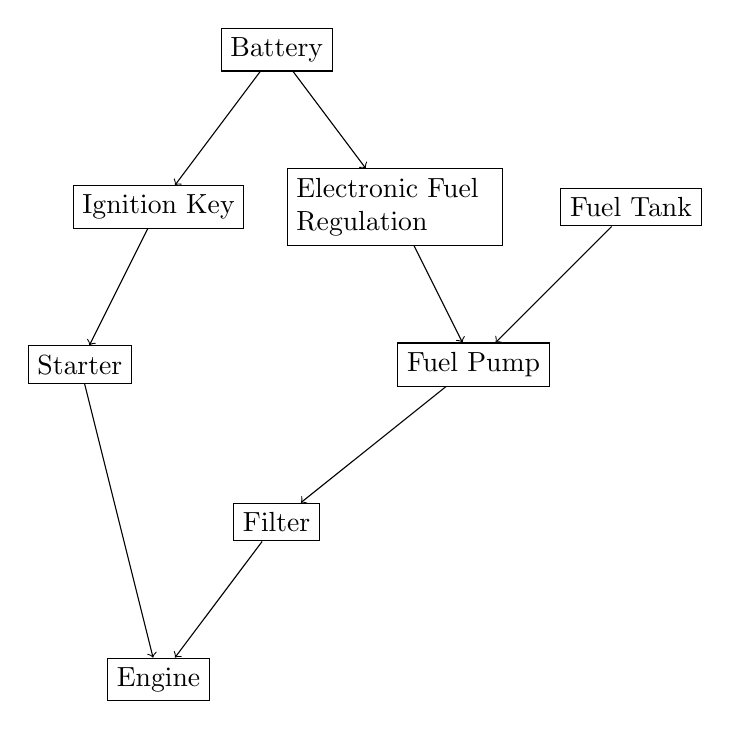
\begin{tikzpicture}
	\node [shape=rectangle,draw=black] (E) at (-1.5,-4) {Engine};
	\node [shape=rectangle,draw=black] (S) at (-2.5,0) {Starter};
	\node [shape=rectangle,draw=black] (F) at (0,-2) {Filter};
	\node [shape=rectangle,draw=black] (FP) at (2.5,0) {Fuel Pump};
	\node [shape=rectangle,draw=black] (FT) at (4.5,2) {Fuel Tank};
	\node [shape=rectangle,draw=black] (I) at (-1.5,2) {Ignition Key};
	\node [text width=2.5cm,shape=rectangle,draw=black] (EFR) at (1.5,2) {Electronic Fuel Regulation};
	\node [shape=rectangle,draw=black] (B) at (0,4) {Battery};
	
	\path [->] (B) edge node {} (I);
	\path [->] (B) edge node {} (EFR);
	\path [->] (I) edge node {} (S);
	\path [->] (S) edge node {} (E);
	\path [->] (FT) edge node {} (FP);
	\path [->] (FP) edge node {} (F);
	\path [->] (F) edge node {} (E);
	\path [->] (EFR) edge node {} (FP); 
\end{tikzpicture}

\begin{align*}
&P(Battery) &&= 0.9\\
&P(\neg Battery) &&= 0.1\\
&\\
&P(Ignition Key|Battery) &&= 0.9\\
&P(\neg Ignition Key| Battery) &&= 0.1\\
&\\
&P(Electronic Fuel Regulation|Battery) &&= 0.9\\
&P(\neg Electronic Fuel Regulation| Battery) &&= 0.1\\
&\\
&P(Fuel Tank) &&= 0.9\\
&P(\neg Fuel Tank) &&= 0.1\\
&\\
&P(Starter| Ignition Key) &&= 0.9\\
&P(\neg Starter | Ignition Key) &&= 0.1\\
&\\
&P(Fuel Pump | Electronic Fuel Regulation \land Fuel Tank) &&= 0.9\\
&P(\neg Fuel Pump | Electronic Fuel Regulation \land Fuel Tank) &&= 0.1\\
&\\
&P(Filter | Fuel Pump) &&= 0.9\\
&P(\neg Filter | Fuel Pump) &&= 0.1\\
&\\
&P(Engine | Starter \land Filter) &&= 0.9\\
&P(\neg Engine | Starter \land Filter) &&= 0.1\\
\end{align*}


\aufgabe{Exercise 9.4: (Bayesian Probabilities)}

\begin{align*}
&P(Smuggler) &&= 0.01\\
&P(\neg Smuggler) &&= 0.99\\
&\\
&P(BarkingDog | Smuggler) &&= 0.8\\
&P(\neg BarkingDog | Smuggler) &&= 0.2\\
&P(BarkingDog | \neg Smuggler) &&= 0.05\\
&P(\neg BarkingDog | \neg Smuggler) &&= 0.95\\
&\\
&P(Sweating | \neg Smuggler \land  \neg Fieber) &&= 0.00\\
&P(Sweating |  Smuggler \land \neg Fieber) &&= 0.4\\
&P(Sweating |  Smuggler \land Fieber) &&= 0.8\\
&P(Sweating |  \neg Smuggler \land Fieber) &&= 0.6\\
&\\
&P(Fieber) &&= 0.013\\
&P(\neg Fieber) &&= 0.987\\
\end{align*}

Berechnen weiterer Wahrscheinlichkeiten:
\begin{align*}
&P(Smuggler | BarkingDog)\\
&\\
\end{align*}
\begin{align*}
&P(Sweating)\\
&\\
\end{align*}
\begin{align*}
&P(Smuggler | BarkingDog \land Sweating)\\
&\\
\end{align*}

\end{document}
